% If you are LaTeX 2.09 user:
% \documentstyle[twocolumn,ncsp17,a4paper]{article}
%
\documentclass[a4paper]{article}
\usepackage[colorlinks, urlcolor=blue,
	pdffitwindow, bookmarksopen,
	filecolor=blue,
	bookmarksopenlevel=0,
	pdfpagelayout=SinglePage, dvipdfm]{hyperref}
\usepackage{ncsp20} %% !! Strongly recommended to use it
\usepackage{color}
\usepackage{graphicx}
\usepackage{multicol}
\usepackage{geometry}
\usepackage{here}
\usepackage{caption}
\usepackage{indentfirst} %なぜか字下げされなくなったので強制させる

\geometry{left=20mm,right=20mm,top=0mm,bottom=12mm}
%topは0にしても微妙に空く、それ以外はきっちり詰まる

\newenvironment{Figure}
  {\par\medskip\noindent\minipage{\linewidth}}
  {\endminipage\par\medskip}
  
%セクションの前後の空白を詰める
\newcommand{\aftersection}{\vspace{-5pt}}
\newcommand{\beforesection}{\vspace{-10pt}}
\newcommand{\beforecaption}{\vspace{-10pt}}

\begin{document}
\name{}
\address{}
\title{Robust and aesthetic colorization for rough sketches}
\maketitle

\vspace{-70pt} % TODO タイトルと本文の間を詰める
\begin{center}
    \begin{tabular}[t]{c}
    {\large Natsuki Ogino}\footnotemark[1]
    \and 
    {\large Kazumasa Horie}\footnotemark[2]
    \and 
    {\large Amagasa Toshiyuki}\footnotemark[2]
    \end{tabular}
\end{center}
\footnotetext[1]{
Graduate School of Science and Technology Degree Programs, University of Tsukuba, 1-1-1 Tennodai, Tsukuba, Ibaraki, 305-8577, Japan.\\
E-mail: ogino.natsuki.tm@alumni.tsukuba.ac.jp}
\footnotetext[2]{
Center for Computational Sciences, University of Tsukuba, 1-1-1 Tennodai, Tsukuba, Ibaraki, 305-8577, Japan.\\
Phone: 029-855-5385
E-mail: \{horie, amagasa\}@cs.tsukuba.ac.jp}

\vspace{-10pt} % TODO タイトルと本文の間を詰める
\begin{figure*}[htbp]
\begin{center}
%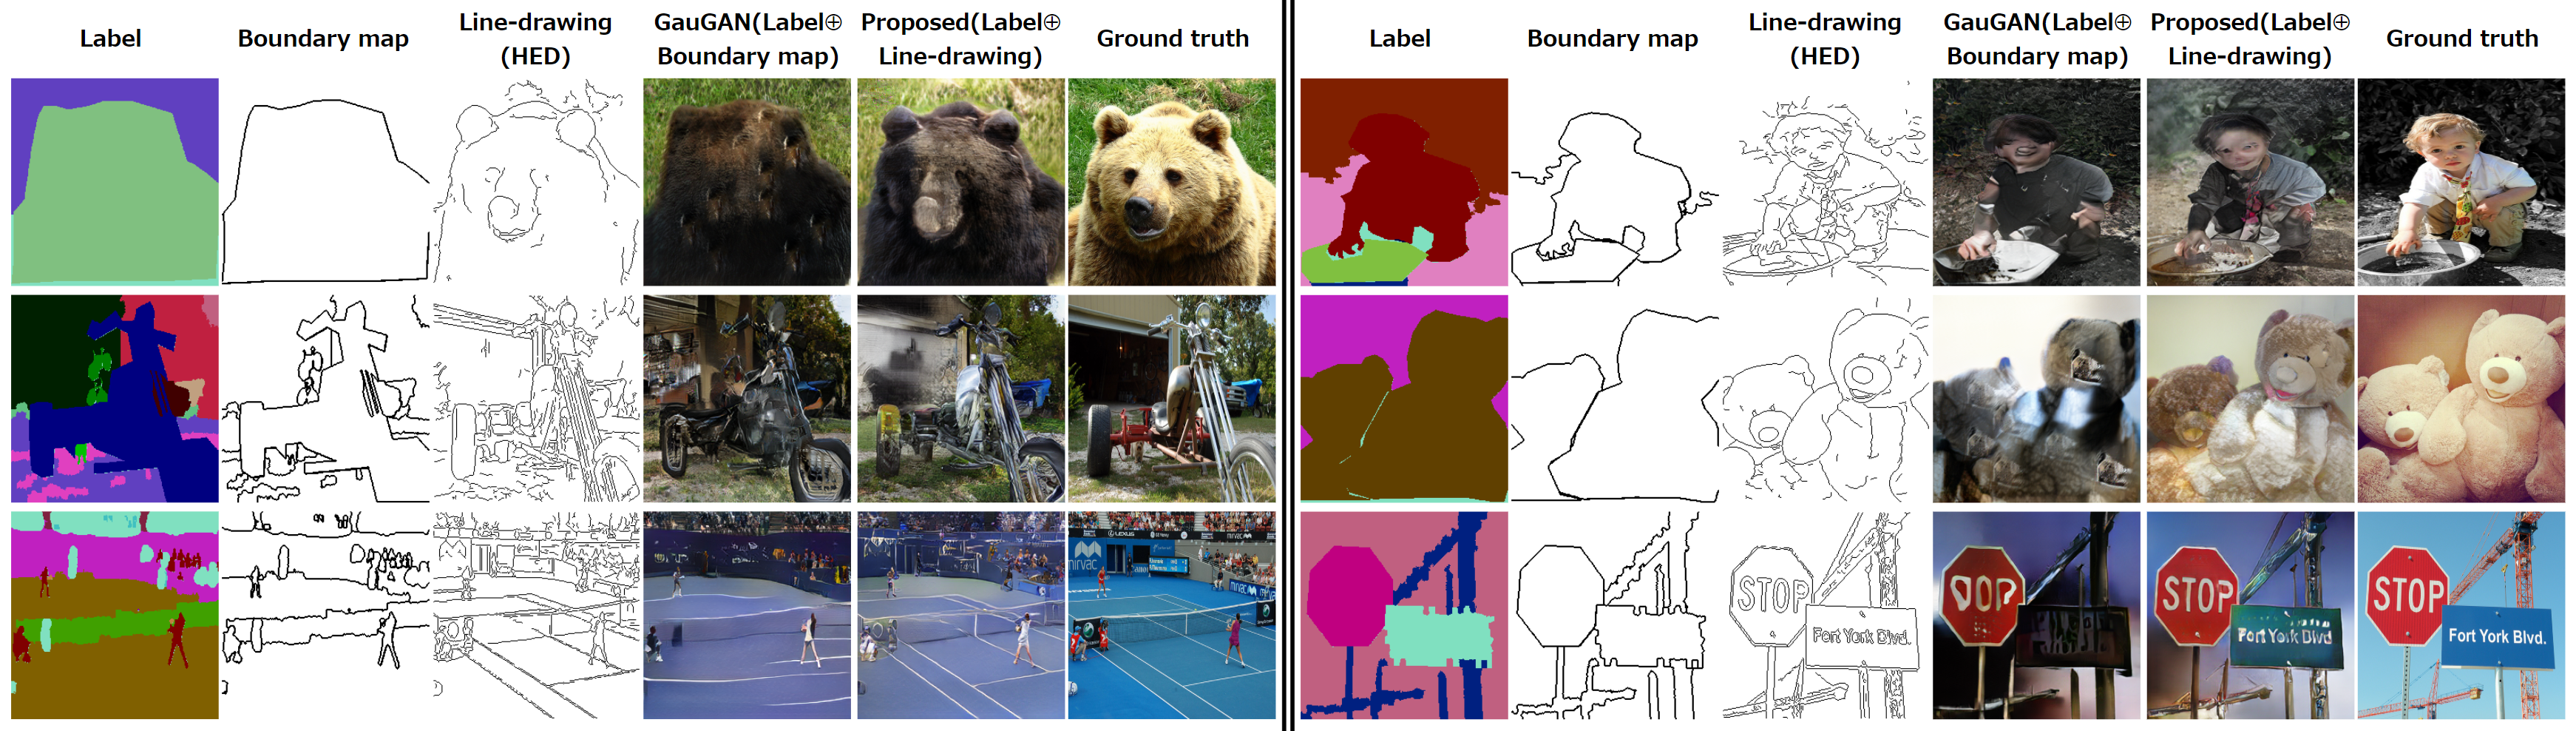
\includegraphics[width=\linewidth]{cherry_pick4.png}
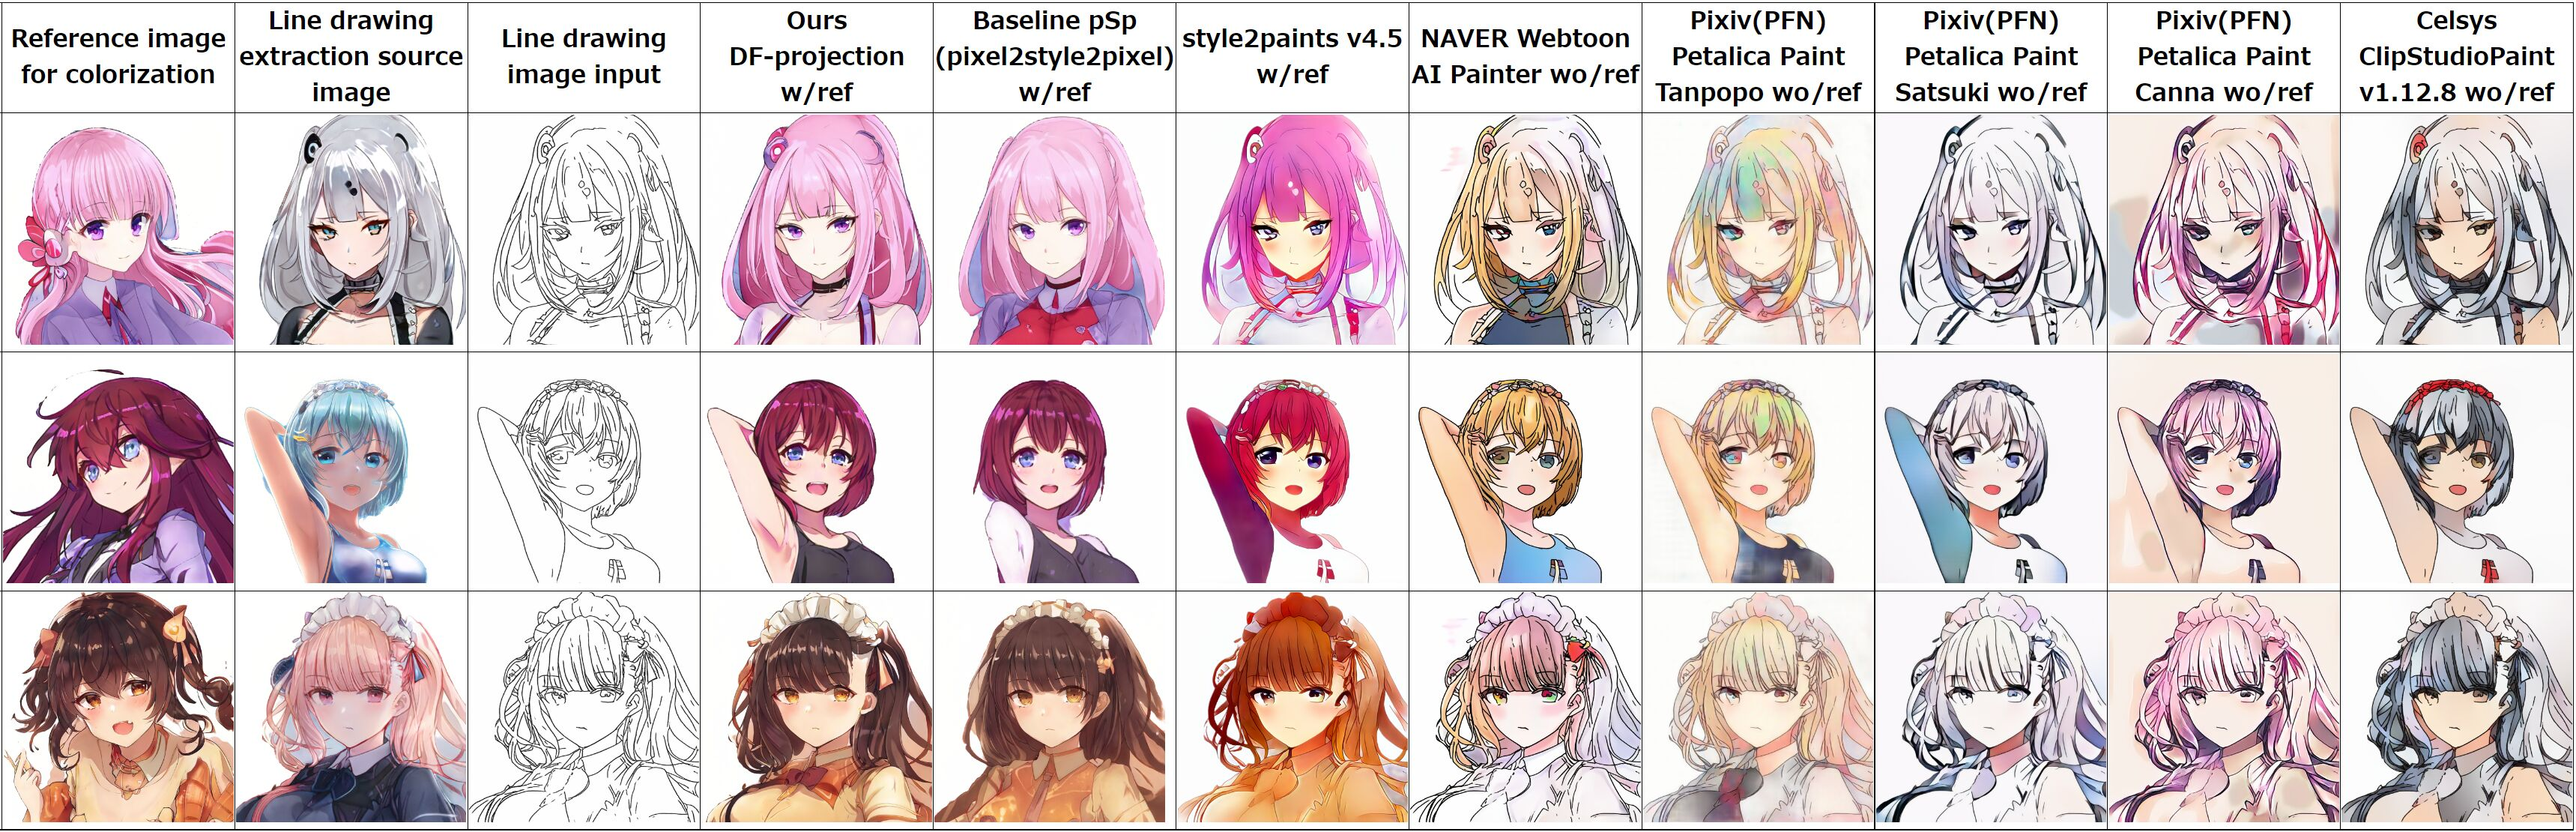
\includegraphics[width=\linewidth]{compare.jpg}
\vspace{-20pt}
\caption{Colorization results of proposed, baseline, and comparative methods}
 \label{figure:results}
\end{center}
\end{figure*}

\vspace{-25pt}
\begin{multicols}{2}
\section*{Objective}
\aftersection
Synthesizing photo-realistic images from semantic layout is highly demanded in the several entertainment fields. Recently, the researches proposed the novel semantic image synthesis methods, named GauGAN~\cite{spade}, and showed its high generation performance. However, we found that GauGAN cannot generate the image of complicated and highly-structured objects, such as the face (Figure~\ref{figure:results}). These objects are usually represented using a single label in the semantic images; therefore, GauGAN cannot grasp its structure from the semantic images. This problem can be solved by adding new semantic labels stands for each part, such as eyes, nose, and mouth; however, this change is undesirable because it significantly increases the user's workload.

Based on the above, the purpose of this research is to develop a GauGAN-based model that can generate the image of highly-structured objects without much increasing the user's workload.

\beforesection
\section*{Methods}
%horie: 従来手法と比べてモデルがどのように変わったかを示す図を入れる// ここ直しておいてください.
%natsuki: 文章の途中で2段組みに切り替えているのでfigure環境でなくFigure環境を使う必要がありました。直しました。
%horie: 荻野君,Fig1のキャプションなんですが,Result(Label+...)となっているとどっちがvanilla GauGANかわかりにくいので,GauGAN(Label+boundary), Proposed(Label+line drawing)のように変更してください.また,HEDmapもline drawings(HED)に変更してください.一回消えます.新しい図近似してくれたのはいいんだけど,ちょっとオーバーフィッティングなのが気になる.指数関数近似できないかな?お願いしますは    い
%natsuki: 指数関数でフィッティングしたものに変更しました。
%Fig. → Figure に統一しました。
%メールの変更点に加え、

\vspace{-40pt}

\begin{Figure}
\begin{center}
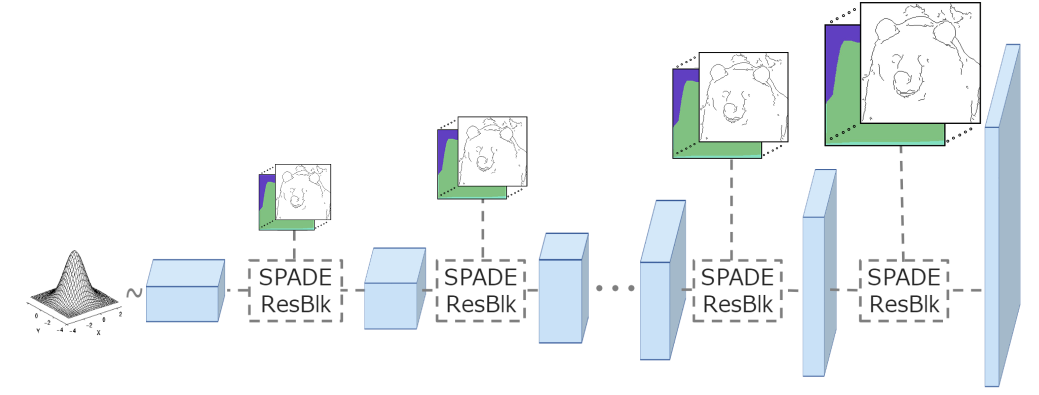
\includegraphics[width=70mm]{trick.png}
\beforecaption
\captionof{figure}{Architecture diagram of our proposed method}
\label{figure:trick}
\end{center}
\end{Figure}

The simplest way to help grasp the structure of the object is by adding information about them as input.
In this research, we chose line drawings as additional information. Drawing lines is not time-consuming and does not require many workloads, compared to preparing semantic images. Besides, these line drawings have enough information to identify the structure of the objects.
Figure~\ref{figure:trick}. shows the structure of the improved GauGAN. We added one input layer for line drawings. 

\beforesection
\section*{Results}
\aftersection

To evaluate the performance of our proposed method, we conducted a comparison experiment with vanilla GauGAN. In this experiment, we used 118,000 training images and 5,000 validation images from the CoCO-Stuff dataset and used "Holistically-Nested Edge Detection" (HED)~\cite{hed} to extract line drawings from these images.  The generation performance was evaluated by the Fréchet Inception Distance (FID) score, which is a distance between the distribution of generated and real images.

\begin{Figure}
\begin{center}
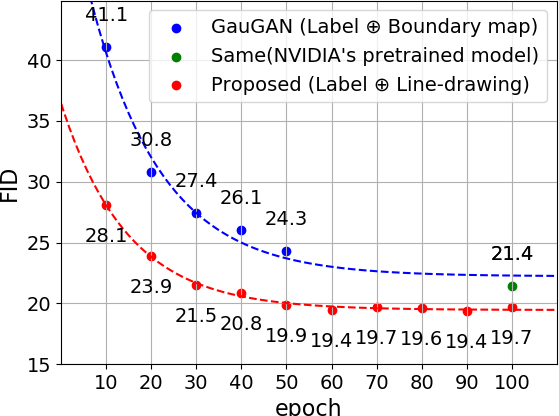
\includegraphics[width=70mm]{fid5.png}
\beforecaption
\captionof{figure}{The relation between the number of training iteration and the FID score}
\label{figure:fid}
\end{center}
\end{Figure}

In contrast to the vanilla GauGAN, Figure~\ref{figure:fid} shows that the FID score of our proposed method rapidly decreased through training and converged less 20.
Besides, Figure~\ref{figure:results}. shows that our proposed methods can generate the image of highly-structured objects that vanilla GauGAN cannot handle.

These results indicate that the line drawings have enough information about the structure and help simplify the relationship between the semantic and realistic images.

\beforesection
\section*{Conclusions}
\aftersection

In this research, we proposed a GauGAN-based image synthesis model that can handle highly-structured objects.
By using line drawings as additional information for the model, the drastic improvement has been achieved without increasing considerable workloads. 

In the camera-ready paper, we will show the comparison with other image synthesis methods and several examples where the proposed method fails. Besides, we will consider how much the line should be required to grasp the structure of the objects.

\vspace{-20pt}
% Reference
\begin{thebibliography}{9}
\bibitem{spade}
T. Park, et al., "Semantic Image Synthesis with Spatially-Adaptive Normalization", Proceedings of Computer Vision and Pattern Recognition, 2019. 
\bibitem{hed}
S. Xie and Z. Tu, "Holistically-Nested Edge Detection", International Journal of Computer Vision, 
Vol. 125, Issue 1-3, pp. 3-18, 2017
\end{thebibliography}

\end{multicols}
\end{document}
